\NeedsTeXFormat{LaTeX2e}[1995/12/01]
\documentclass[10pt]{bmc_article}    
\usepackage[usenames]{color}

% Load packages
\usepackage{cite} % Make references as [1-4], not [1,2,3,4]
\usepackage{url}  % Formatting web addresses  
\usepackage{ifthen}  % Conditional 
\usepackage{multicol}   %Columns
\usepackage[utf8]{inputenc} %unicode support
%\usepackage[applemac]{inputenc} %applemac support if unicode package fails
%\usepackage[latin1]{inputenc} %UNIX support if unicode package fails
\urlstyle{rm}
 
%%%%%%%%%%%%%%%%%%%%
%% Karro macros   %%
%%%%%%%%%%%%%%%%%%%%
\newcommand{\peace} {{\small PEACE}}
\newcommand{\wcd} {{\small WCD}}
\newcommand{\capthree} {{\small Cap3}}
\newcommand{\easycluster} {{\small EasyCluster}}
\newcommand{\estsim}{{\small ESTSim}}
\newcommand{\metasim} {{\small MetaSim}}
\newcommand{\tgicl} {{\small TGICL}}
\newcommand{\east} {{\small EAST}}
\newcommand{\velvet}{{\small Velvet}}
\newcommand{\mira}{{\small Mira3}}
\newcommand{\pave} {{\small PAVE}}
\newcommand{\peast}{{\small PEACE+EAST}}
 
%%%%%%%%%%%%%%%%%%%%%%%%%%%%%%%%%%%%%%%%%%%%%%%%%	
%%                                             %%
%%  If you wish to display your graphics for   %%
%%  your own use using includegraphic or       %%
%%  includegraphics, then comment out the      %%
%%  following two lines of code.               %%   
%%  NB: These line *must* be included when     %%
%%  submitting to BMC.                         %% 
%%  All figure files must be submitted as      %%
%%  separate graphics through the BMC          %%
%%  submission process, not included in the    %% 
%%  submitted article.                         %% 
%%                                             %%
%%%%%%%%%%%%%%%%%%%%%%%%%%%%%%%%%%%%%%%%%%%%%%%%%                     

\usepackage{graphicx}
%\def\includegraphic{}
%\def\includegraphics{}


\setlength{\topmargin}{0.0cm}
\setlength{\textheight}{21.5cm}
\setlength{\oddsidemargin}{0cm} 
\setlength{\textwidth}{16.5cm}
\setlength{\columnsep}{0.6cm}

\newboolean{publ}

%%%%%%%%%%%%%%%%%%%%%%%%%%%%%%%%%%%%%%%%%%%%%%%%%%
%%                                              %%
%% You may change the following style settings  %%
%% Should you wish to format your article       %%
%% in a publication style for printing out and  %%
%% sharing with colleagues, but ensure that     %%
%% before submitting to BMC that the style is   %%
%% returned to the Review style setting.        %%
%%                                              %%
%%%%%%%%%%%%%%%%%%%%%%%%%%%%%%%%%%%%%%%%%%%%%%%%%%
 

%Review style settings
\newenvironment{bmcformat}{\begin{raggedright}\baselineskip20pt\sloppy\setboolean{publ}{false}}{\end{raggedright}\baselineskip20pt\sloppy}

%Publication style settings
%\newenvironment{bmcformat}{\fussy\setboolean{publ}{true}}{\fussy}



% Begin ...
\begin{document}
\begin{bmcformat}

\title{EAST: {\underline E}xpression Fragment {\underline A}ssembly from {\underline S}panning {\underline T}rees}

%%%%%%%%%%%%%%%%%%%%%%%%%%%%%%%%%%%%%%%%%%%%%%
%%                                          %%
%% Enter the authors here                   %%
%%                                          %%
%% Ensure \and is entered between all but   %%
%% the last two authors. This will be       %%
%% replaced by a comma in the final article %%
%%                                          %%
%% Ensure there are no trailing spaces at   %% 
%% the ends of the lines                    %%     	
%%                                          %%
%%%%%%%%%%%%%%%%%%%%%%%%%%%%%%%%%%%%%%%%%%%%%%


\author{Yuan Zhang$^1$
  \email{Yuan Zhang - zhangy9@muohio.edu}
  \and
  Dhananjai M Rao$^1$
  \email{Dhananjai Rao - raodm@muohio.edu}
  \and
  Mufit Ozden$^1$
  \email{Mufit Ozden - ozdenm@muohio.edu}
  \and
  Jens Mueller$^2$
  \email{Jens Mueller - muellej@muohio.edu}
  \and
  Praveen Kumar Raj Kumar$^4$
  \email{Praveen Kumar - rajkump@muohio.edu}
  \and
  Chun Liang\correspondingauthor$^{1,3}$
  \email{Chun Liang\correspondingauthor - liangc@muohio.edu}
  and
  John E. Karro\correspondingauthor$^{1,4,5}$
  \email{John E. Karro\correspondingauthor - karroje@muohio.edu}
}

%%%%%%%%%%%%%%%%%%%%%%%%%%%%%%%%%%%%%%%%%%%%%%
%%                                          %%
%% Enter the authors' addresses here        %%
%%                                          %%
%%%%%%%%%%%%%%%%%%%%%%%%%%%%%%%%%%%%%%%%%%%%%%

\address{
  \iid(1)Department of Computer Science and Software Engineering,  \\
  \iid(2)Informational Technology Services\\
  \iid(3)Department of Botanty, \\
  \iid(4)Department of Microbiology, \\
  \iid(5)Department of Statistics, Miami University, Oxford OHIO, USA
}

\maketitle

%%%%%%%%%%%%%%%%%%%%%%%%%%%%%%%%%%%%%%%%%%%%%%
%%                                          %%
%% The Abstract begins here                 %%
%%                                          %%
%% The Section headings here are those for  %%
%% a Research article submitted to a        %%
%% BMC-Series journal.                      %%  
%%                                          %%
%% If your article is not of this type,     %%
%% then refer to the Instructions for       %%
%% authors on http://www.biomedcentral.com  %%
%% and change the section headings          %%
%% accordingly.                             %%   
%%                                          %%
%%%%%%%%%%%%%%%%%%%%%%%%%%%%%%%%%%%%%%%%%%%%%%


\begin{abstract}
\end{abstract}



\ifthenelse{\boolean{publ}}{\begin{multicols}{2}}{}


%%%%%%%%%%%%%%%%%%%%%%%%%%%%%%%%%%%%%%%%%%%%%%
%%                                          %%
%% The Main Body begins here                %%
%%                                          %%
%% The Section headings here are those for  %%
%% a Research article submitted to a        %%
%% BMC-Series journal.                      %%  
%%                                          %%
%% If your article is not of this type,     %%
%% then refer to the instructions for       %%
%% authors on:                              %%
%% http://www.biomedcentral.com/info/authors%%
%% and change the section headings          %%
%% accordingly.                             %% 
%%                                          %%
%% See the Results and Discussion section   %%
%% for details on how to create sub-sections%%
%%                                          %%
%% use \cite{...} to cite references        %%
%%  \cite{koon} and                         %%
%%  \cite{oreg,khar,zvai,xjon,schn,pond}    %%
%%  \nocite{smith,marg,hunn,advi,koha,mouse}%%
%%                                          %%
%%%%%%%%%%%%%%%%%%%%%%%%%%%%%%%%%%%%%%%%%%%%%%




%%%%%%%%%%%%%%%%
%% Background %%
%%
  \section*{Introduction}

  The {\it de novo} assembly of RNA transcripts is an important and
  computationally challenging problem, made more difficult by the
  advent of Next Generation Sequencing technologies such as 454 and
  Illumina \cite{Nagaraj07,Rao10}.  Upon completion of
  transcriptome-sequencing, the investigator is left with a large set
  of sequence fragments but no ordering or transcript association
  information.  These fragments must be clustered by transcript and
  assembled before the sequencing output can be truly useful.  {\it de
    novo} assembly tools assemble the transcript out of the fragments
  without using genomic sequence information.  {\it de novo} tools are
  obivously necessary when working with a genome that is unsequenced
  or poorly annotated, but are also useful when there is limited
  knowledge of gene splice sites \cite{Birol09,Robertson10}, they can
  aid in the discovery of novel biological processes
  (e.g. transplicing and fusion transcript) \cite{Mitelman07,Li10b}, and
    they are invaluable for annotating structural variations not
    contained within the genome \cite{Li08}.



  \vspace{3mm}

  The problem of {\it de novo} transcript assembly has been addressed
  a number of times in the literature, with initial approaches
  concentrating on the longer reads produced by traditional Sanger
  Sequencing techniques, and newer approaches looking at produces of
  Next Generation Sequencing (NGS) technologies.  A list of popular
  tools addressing these problems include \capthree, \tgicl, \velvet,
  and \mira, each excelling within their own context
  \cite{Huang99,Pertea03,Chevreux04,Zerbino08}.  \capthree\/ and
  \tgicl\/ use alignment-based strategies that produce high quality
  results when applied to the output of Sanger sequencing
  technologies.  \velvet, based on the modeling of the problem with
  {\it de bruijn} graphs, was designed to handle short read sequences.
  \mira\/ is a multi-pass DNA assembler based on an
  overlap-layout-consensus strategy that also has an increased ability
  to assemble {\it hybrid sets}: sets formed by the mixture of
  sequencing results from multiple technologies \cite{MiraWeb}.

\vspace{3mm}

In this paper we present \east: a tool for the assembly of
Sanger, NGS and hybrid data with the capacity to incorporate quality
scores when available.  \east\/ is based on a novel Minimum Spanning
Tree (MST) approach to compute assembly.  The tool works in tandem
with the \peace\/ clustering tool \cite{Rao10}: \peace\/ clusters
fragments by transcript and produces the initial MSTs that will serve
as the basis for the \east\/ algorithm.  In this paper we present a
comparison of \east\/ against \capthree, \tgicl, \velvet, and
\mira\/ on both Sanger and NGS sequences, showing that \peast\/
generates the best quality results in the fastest runtime for Sanger
sequences.  Although certain tools out-perform \peace\/ under
specific conditions, we show that it is the only tool able to produce consistently
higher quality results for Sanger, 454, Illumina, {\it and} hybrid
data sets.  In this paper we discuss the results and relevant
computational methods.  \east\/ has been incorporated into the
\peace\/ clustering tools \cite{Rao10}; it can be installed
and run through a Java-based PEACE GUI available at
www.peace-tools.org.

 
%%%%%%%%%%%%%%%%%%%%%%%%%%%%
%% Results and Discussion %%
%%
\section*{Results and Discussion}

In assessing result quality, we must view the \peace\/ clustering tool
\cite{Rao10} and \east\/ as a combined process.  While most assembly
tools integrate these two jobs, \east\/ assumes clustering has been
performed and requires the \peace\/ MST output.  Hence for purposes of
the following section, we consider them as a single tool \peast, and
assess the quality of these results.

\vspace{3mm}

In order to assess the quality of (\peace\/ +) \east\/ results, we compared
against four prominent assembly tools: \capthree, \tgicl,
\mira, and \velvet\/ \cite{Huang99,Pertea03,Chevreux04,Zerbino08}.  The tools were tested on data from three
sequencing technologies (Sanger, 454 and Illumina), using both
simulated output obtained from the \estsim\/ and \metasim\/ tools
\cite{Hazelhurst03,Richter08}.  


\subsection*{Measuring Quality}
Our primary measure of quality was the {\bf normalized a-score}, based
on the {\it assembly score} (a-score) used in {\it Liang et al.}
\cite{Liang00}.  For an assembly of some original sequence, the
a-score is defined as:
$$\mbox{($2\times$sequence length) - ($5\times$number of
mismatches) - ($15 \times$number of indels)}$$
with a ``perfect'' score equal to twice the sequence length.  Our
normalized a-score modifies this definition as:
$$\frac{\mbox{($2\times$assembly length) - ($5\times$number of mismatches)
    - ($15\times$number of indels)}}{\mbox{($2\times$sequence
    length)}}$$ with a perfect score equal to 1.  This normalization
allows for the comparison of assembly quality between sequences of
different lengths. Further, using this score we can more accurately
quantify the quality of a partial reconstruction: if we are able to
reconstruct only a portion of a fragment, the normalized a-score will
take full consideration of the quality of the reconstruction, but then
bound the score by the relative size of the reconstruction.
(For example, were a tool only able to reconstruct a
  contig covering one fourth of a transcript -- but able to
  reconstruct that fraction perfectly -- the resulting contig's
  normalized a-score would be $0.25$.)  In addition we look at: the
number of contigs produced by a tool normalized by the number of
transcripts (a value equal to 1 in a perfect reconstruction); the
number of singleton ESTs in the solution (i.e. ESTs unassigned to any
contig and thus, most cases, effectively thrown away), and the runtime
of the tool.

\subsection*{Simulation Results}
Using simulated fragment sets allows us to compare assemblies to
a known correct solution and control parameters in their model
(e.g. base-call error rate) to test the effect of variation.  All sets
were generated from a collection of 100 zebra fish transcripts
obtained from {\it Hazelhurst et al.}  \cite{Hazelhurst08}.  For
simulated Sanger sequences we used the \estsim\/ tool, using its
default model of EST generation when not otherwise specified
\cite{Hazelhurst03}.  For simulated 454 and Illumina sets we used the
\metasim\/ tool, again using their default model to simulate the
errors associated with those technologies \cite{Richter08}. {\bf
  [COMMENT: Will try to add a discussion of, or reference to, the
  default values here.]}

\vspace{3mm}

\noindent {\bf Sanger Sequencing:} We first compare the
  assembly quality of the tools on a Sanger Sequencing model, using
  \east, \capthree, and \tgicl\/, the tools designed to work with
  Sanger sequence.  The quality of any assembly will be directly
  affected by the {\it covreage} of the input: the average number of
  ESTs that cover a based.  Thus we investigate the a-score as a
  function of error rate at different coverage levels.  For each
parameter combination we applied each tool to 30 independent, randomly
generated simulated sets, derived from 15 randomly chosen members of
our zebra fish gene set, reporting the average normalized a-score.  In
Figure~\ref{sangerAscore} we look at normalized a-score as a function
of error rate, fixing coverage at 50, 30 and 10 and varying base read
error rate from 0\% to 6\% for each of the three tools designed for
Sanger Sequencing.  While all three tools perform well when applied to
error free (i.e. impossible) sequencing technology, we find \east\/ to
be considerably more robust to base-call errors than the other tools.
Taking the mid-range coverage value of 30 as an example, at a 1\%
error rate we see \east, \capthree, and \tgicl\/ all achieving an
essentially perfect normalized a-score.  At a 3\% error rate \east\/
maintains its almost perfect normalized a-score, showing a 2\%
improvement over \tgicl\/ and a 21\% improvement over \capthree.  At a
4\% error rate \east\/ still maintains its near-perfect score (showing
a 54\% and 85\% improvement over \capthree\/ and \tgicl\/
respectively).  Even at a 6\% error rate \east\/ is still achieving a
normalized a-score of 0.95 (a 110\% improvement over the next closest
tool, \tgicl\/), meaning that at most 5\% of the bases were left out
of their contigs or were incorrectly reconstructed.


\begin{figure}[htb]
\centerline{\includegraphics[width=6in]{pics.d/ascore_sanger_norm.pdf}}
\caption{Average normalized a-score as a function of base error rate for
  simulated Sanger sequencing.  \east=blue, \capthree=Black,
  \tgicl=green. COMMENT: Need to change figure heading to Normalized a-score.}
\label{sangerAscore}
\end{figure}

In Figure~\ref{contigsSanger} is a
plot of the average number of contigs per gene sequence (left column), and
the number of singletons (right column).  For the first we observe that all tools have
comparable results for lower error rates, but only \east\/ is able to
maintain the low score with increasing error rates -- generating a
perfect score in almost every case.  In minimizing the
number of singletons, we find that \east\/ does a better job than
\capthree\/ for error rates larger than $2\%$, while \tgicl\/ does a
better job that \east\/ for error rates larger than $4\%$ to $5\%$.

\begin{figure}[htb]
\begin{minipage}{3in}
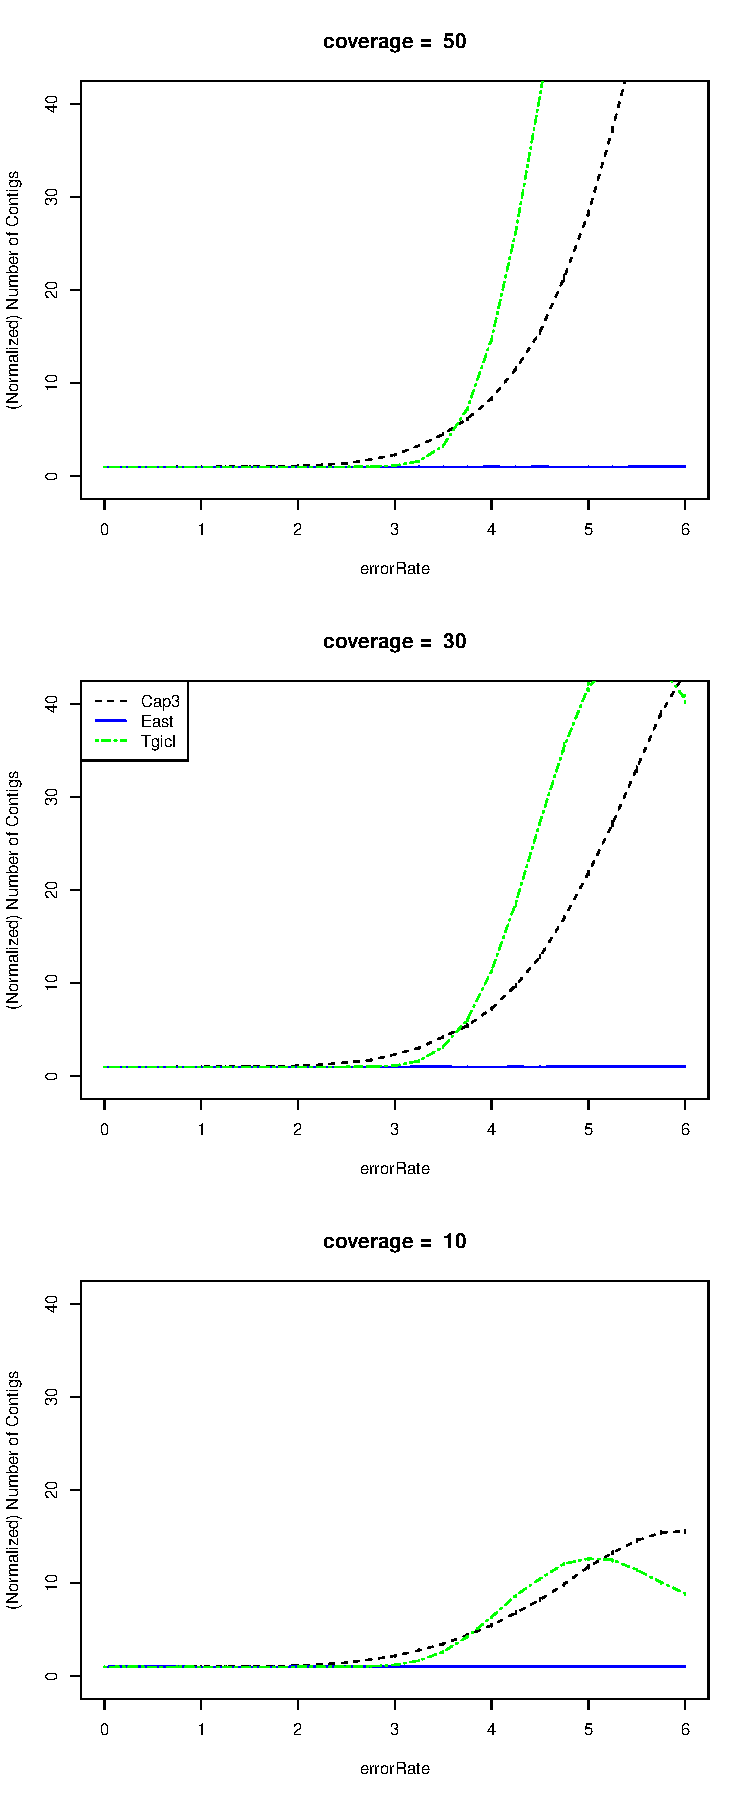
\includegraphics[width=3in]{pics.d/numContigs_sanger.pdf}
\end{minipage}
\begin{minipage}{3in}
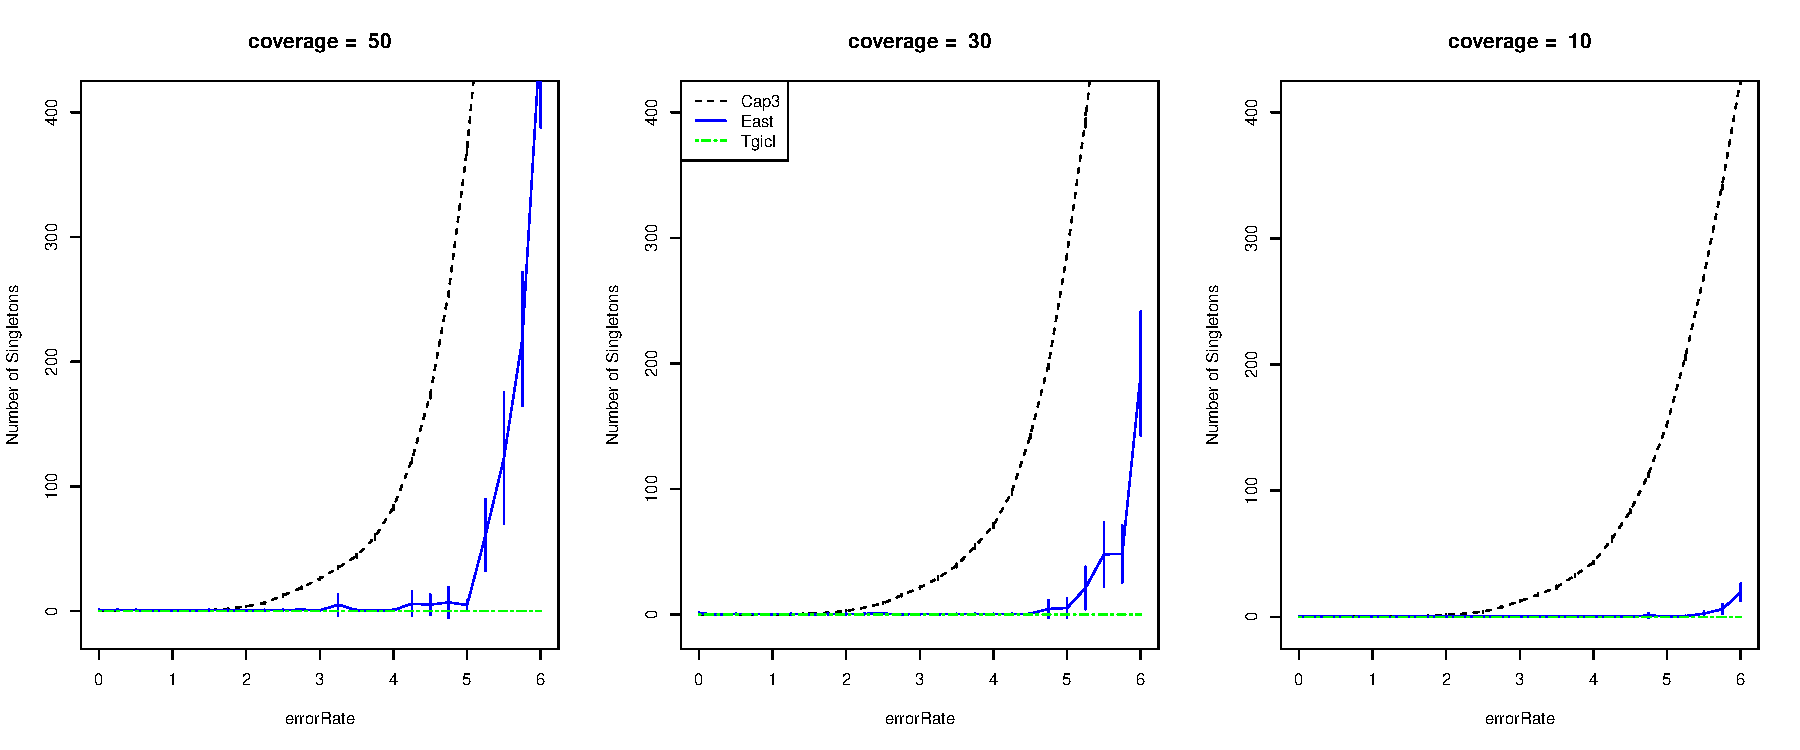
\includegraphics[width=3in]{pics.d/numSingle_sanger.pdf}
\end{minipage}
\caption{Number of contigs (normalized to the number of transcripts)
  and number of singletons as a function of base-call error
  rate for simulated Sanger sequencing.  \east=blue, \capthree=Black,
  \tgicl=green.  (Number of singletons for
  \velvet\/ and \mira\/ not shown.)}
\label{contigsSanger}
\end{figure}


\noindent {\bf Next Generation Sequences:} In
Figure~\ref{nextgenAscore} we compare the normalized a-score for
simulated 454 and Illumina outputs (with sequence lengths averaging
250 and 62 bp respectively).  For these tests we varied coverage
levels but otherwise continued to use the default Metasim model
\cite{Richter08}.  On 454 data we see significant improvement in
results quality in \east\/ for all levels of coverage.  On Illumina
data we see that \east\/ is competitive with \velvet\/ at higher
coverages, though is unable to match that tool when coverage is
sparse.

\begin{figure}[htb]
\centerline{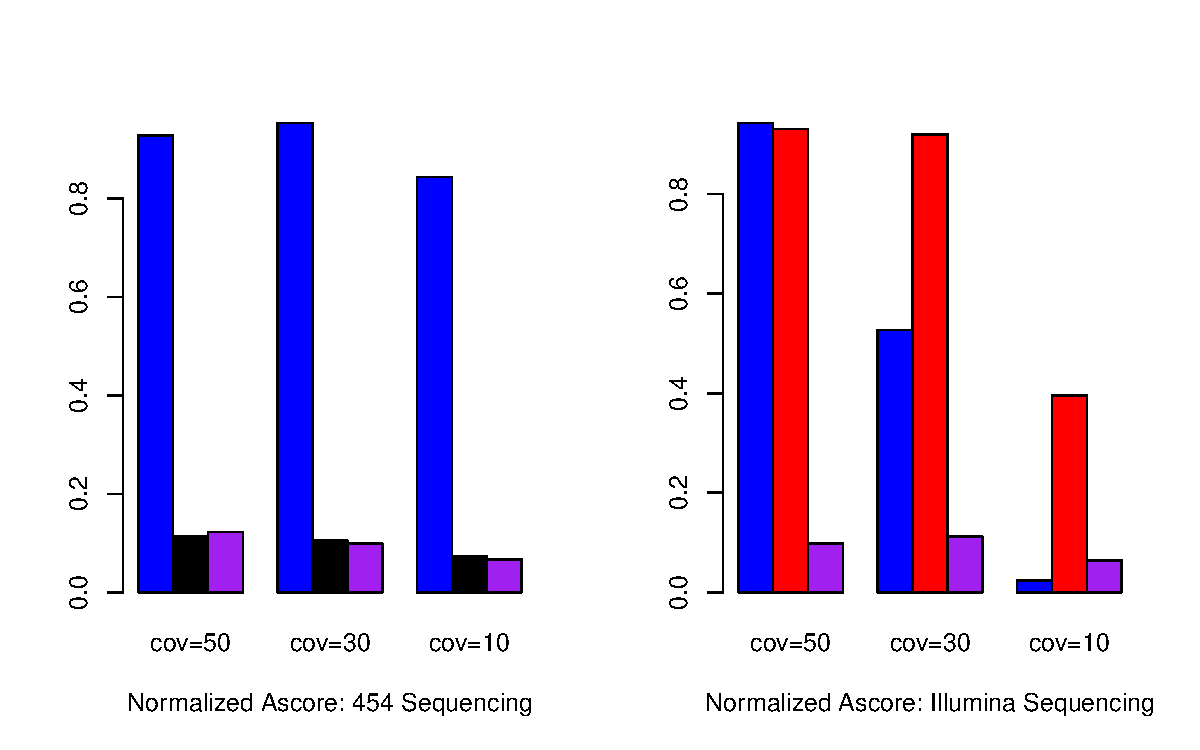
\includegraphics[width=6in]{pics.d/ascore_nxtgen.pdf}}
\caption{Comparative normalized a-scores for 454 and Illumina sequence
  output, using the \metasim default model at different levels
  of coverage.  \east=blue, \capthree=Black, \tgicl=green.  }
\label{nextgenAscore}
\end{figure}

\noindent {\bf Hybrid:} In Figure~\ref{hybridAscore} we look at the
quality of results derived from applying each tool to a hybrid data
set of Sanger (40\%), 454 (40\%) and Illumina (20\%) sequences, again
showing normalized a-score as a function of base-call error rate in
the Sanger portion.  Here we observe \east\/ matching or outperforming
\capthree\/ and \mira\/ at moderate to high coverages.  At a coverage
level of 50, \east\/ maintains a normalized a-score hovering around
0.85 at all error levels (showing a 54\% improvement over \mira\/ at a
3\% base-call error rate).  \east\/ actually improves its performance
at a coverage level of 30 (hovering around a normalized a-score of
0.95, showing a 142\% improvement over \mira\/ at the 3\% base-call error
rate), an oddity we attribute to the decreased absolute number of NGS
sequences with the smaller coverage.  At a coverage level of 10
\east's normalized a-score is around 0.37 -- performing considerably
worse than \mira\/ at low error rates (e.g. 0.94 v. 0.40 for
error-free bases), but showing a 52\% improvement over \mira\/ at the
3\% error rate mark and in general showing increased robustness to
error.  Remarkably, it is only in this situation that \capthree\/ is
competitive, with that tool achieving a normalized a-score of 0.62
(v. \east's 0.37) for the 3\% base-call error rate, but loosing out to
\east\/ at greater than a 4.5\% base-call error rate -- a situation
likely due to \east's problems with the 62 bp Illumina sequences (see
below).

\begin{figure}[htb]
\centerline{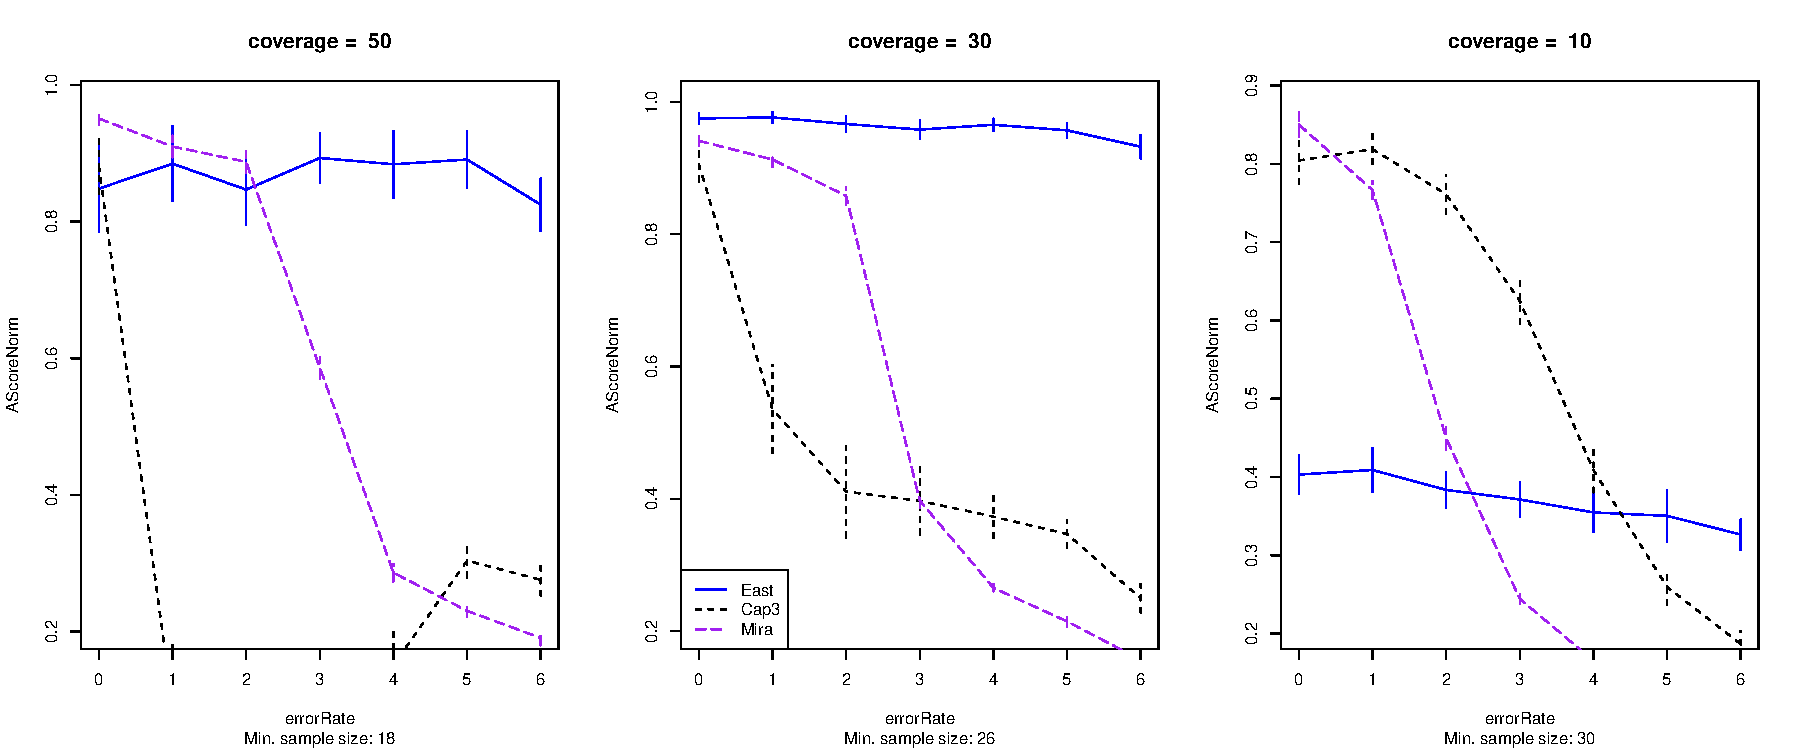
\includegraphics[width=6in]{pics.d/ascore_hybrid.pdf}}
\caption{Comparative normalized a-scores for a hybrid set consisting
  of Sanger, 454 and Illumina sequence output, varying the base-call
  error rate for Sanger sequences and using the MetaSim default model
  for the 454 and Illumina sequences.  Each data set tested was
  composed of 40\% Sanger Sequences, 40\% 454 Sequences, and 20\%
  Illumina sequences.  \east=blue, \capthree=Black, \tgicl=green,
  \velvet=red, \mira=purple.}
\label{hybridAscore}
\end{figure}

\noindent {\bf Tool Runtime:} In Figures~\ref{runtime.fixed} we see
the average runtime for each of the experiments reflected in
Figures~\ref{sangerAscore}-\ref{hybridAscore} for a coverage of 30
(continuing to report the combined runtime of \peace+\east), while in
Figure~\ref{runtime.coverage} we look at the average runtime for each
tool when applied to simulated data sets generated from a single zebra
fish gene at varying levels of coverage.  For Sanger sequences we
see marked improvement of (\peace+)\east\/ over all other tools for
almost all coverage levels: for the smallest set (coverage = 10)
\east\/ has 1.9 speedup over \capthree\/ and a 3.9 speedup over
\tgicl, while at a more moderate size (coverage=50) there are speedups of
4.7 and 8.4.  This returns back down to 3.0 and 5.2 at the largest set
tested (coverage = 100), as can be seen in the bump around a coverage
of 85 in Figure~\ref{runtime.coverage}.  We are unable to
superficially explain this bump, but have noticed the same effect in
data sets derived from other genes as well.

\vspace{3mm}

\east\/ is less competitive on shorter sequence.  In our simulations,
we find a reduced runtime improvement on the simulated 454 sequences
(averaging 250 bp in length), and a significantly reduced runtime on
the simulated Illumina sequences (exactly 62 bp in length).  However,
as technology advances, the ``short-read'' sequencers are producing
increasingly longer reads: 454 sequencing technology can produce
reads exceeding 400 bp, while Illumina sequences can exceed 100 bp
\cite{Eid09,Li10}.  The loss of runtime in our experiments on 454,
Illumina and the hybrid sequences are due to the shorter sequence
(specifically, the problems with applying the $d^2$ metric to shorter
sequences -- as discussed below), hence are becoming less of an issue
with this increase in short-read fragment length.

\vspace{3mm}

In short, we argue that the high quality of our results still makes
\east\/ an appealing option for 454 and hybrid data (while
acknowledging that \east\/ cannot currently compete with \velvet\/ on pure
Illumina data), and also observe that while it has not been
implemented, the basic \east\/ algorithm will easily admit
parallelization -- thus increasing the practical limit on data set
size.

\begin{figure}[htb]
\centerline{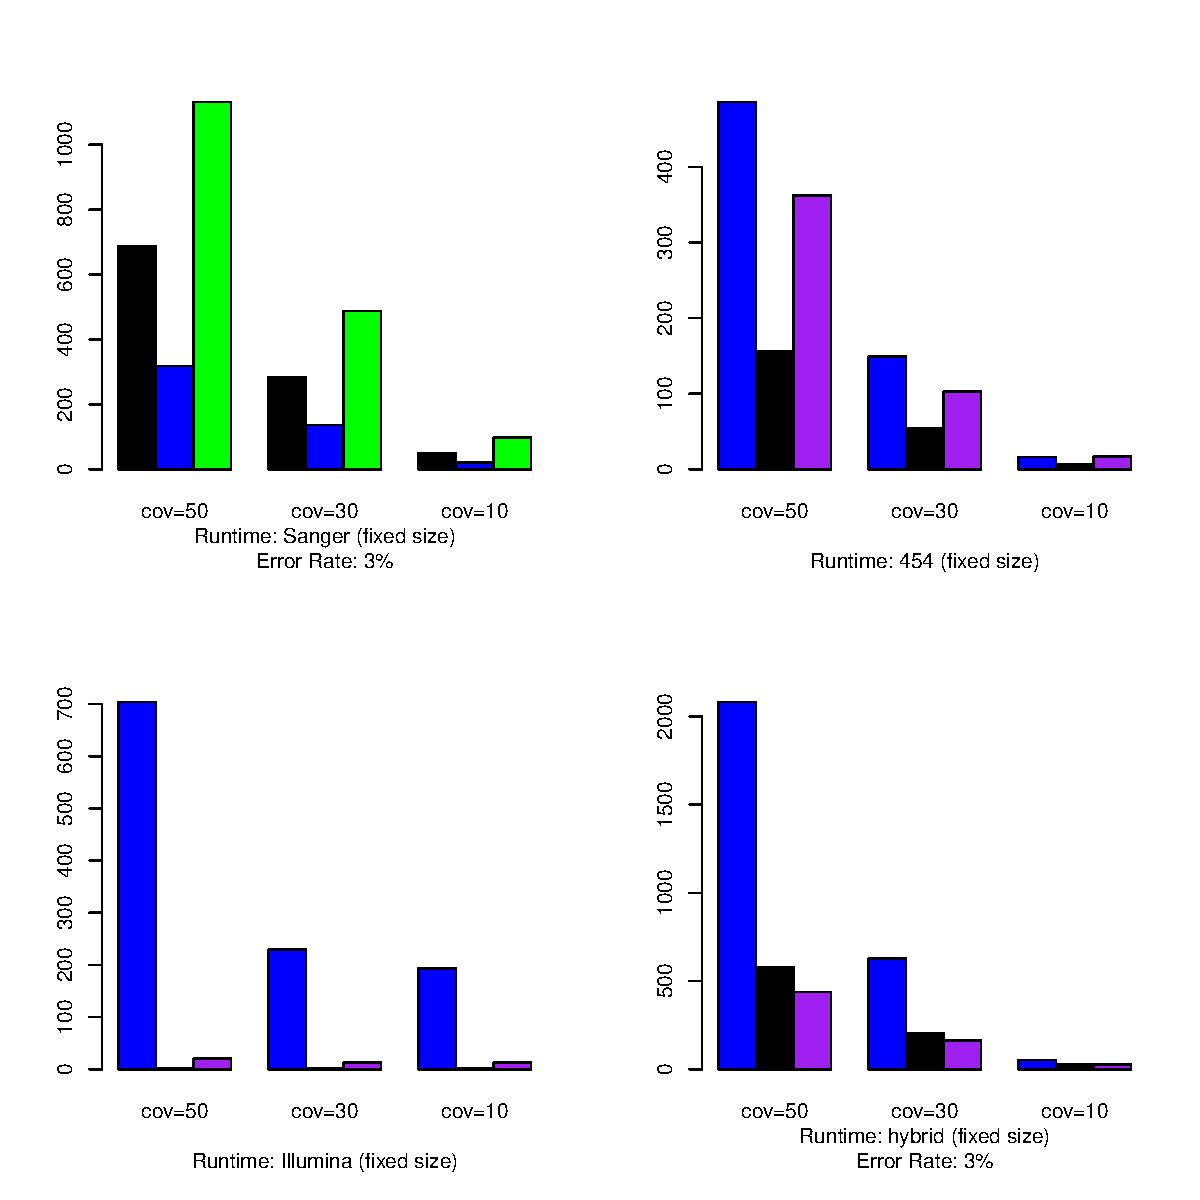
\includegraphics[width=6in]{pics.d/runtime_fixedsize_sanger.pdf}}
\caption{Average runtime per trial when when generating data for
  Figures~\ref{sangerAscore}-\ref{hybridAscore}  when coverage = 30.
  Note that the exceptionally high speed of \velvet\/ on Illumina sequences make the
  red (center) bars in that plot essentially indistinguishable.
  (\peace+)\east=blue, \capthree=Black, \tgicl=green,
  \velvet=red, \mira=purple.}
\label{runtime.fixed}
\end{figure}

\begin{figure}[htb]
\centerline{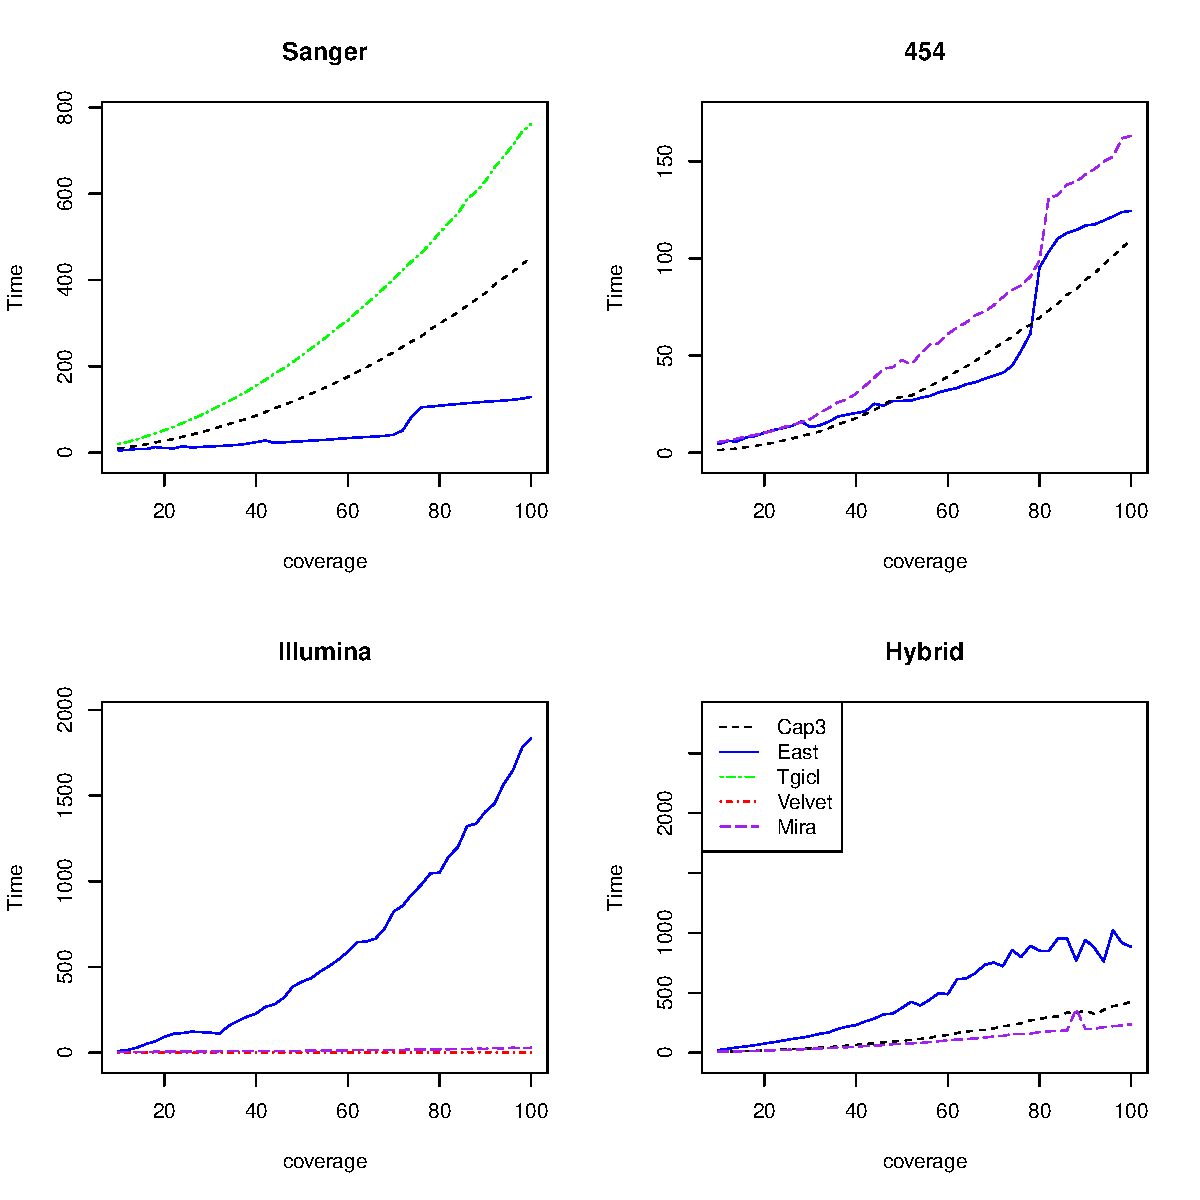
\includegraphics[width=6in]{pics.d/runtime_bycoverage_all.pdf}}
\caption{The average runtime when applying each tool to a simulated
  data set derived from a specific zebrafish transcript of length
  14,625 bp.  As we decrease coverage the number of fragments drops,
  hence illustrating the relationship between tool runtime and
  fragment set size.  Each data point represents the average runtime
  from the application of the tool to at least 30 randomly generated
  simulated sets coming from the transcript at the given level of coverage.
  \peace + \east=blue, \capthree=Black, \tgicl=green,
  \velvet=red, \mira=purple.}
\label{runtime.coverage}
\end{figure}

\noindent{\bf Implementation:} \east\/ has been integrated into the
\peace\/ clustering package \cite{Rao10} and is available for
download from the \peace\/ website ({\bf www.peace-tools.org}).
Users can run the GUI provided by that site, and through it
install both the \peace\/ cluster engine and \east\/ assembly engine
on a local machine or remote server (see Figure~\ref{GUI-fig}).
Initial EST data must be in fasta format, though the tool can print
out the final assembly in fasta, ACE, SAM and BAM formats [NEED TO ADD
CITATION TO THE CONVERSION TOOL].

\begin{figure}[htb]
\centerline{\includegraphics[width=6in]{pics.d/GUI1.pdf}}
\caption{Screen shots of the PEACE GUI.  [COMMENT: Need to improve this.]}
\label{GUI-fig}
\end{figure}

%%%%%%%%%%%%%%%%%%%%%%
\section*{Conclusions}

{\textcolor{blue}{In this manuscript we have described the \east\/ algorithm and we have run a
comparison of the \peast\/ tool combination against popular tools
from the literature.}  When compared against competing tools on simulated
data using the normalized a-score and runtime metrics, the \peast\/ combination of
tools produce the best sequence assemblies for Sanger sequence, the
best tool overall [COMMENT: I need a better way to phrase this --
something to indicate the do better as a whole, even if they don't do
as well as some tools on some sets], and by far the most robust against sequencing
error.  While certain tools may do better than \east\/ in specific circumstances,
none of them do better than EAST on multiple sequencing
technology platforms.  While its speed is slower when applied to short
sequence fragments, the quality of its results more then compensate.}
\vspace{3mm}

As observed in the results section, when applying \east, \capthree,
and \tgicl\/ to Sanger sequenced transcripts with normal to high error
rates, \east\/ consistently out performs all other tools in terms of
the normalized a-score metric (Figures~\ref{sangerAscore},
\ref{runtime.fixed}, and \ref{runtime.coverage}).  We also find that
the number of contigs produced is almost exactly equal to the number
of transcripts represented in the set, regardless of error rate, while
the number of singleton ESTs remains low up to about a 5\% error rate
(Figures~\ref{contigsSanger}).  The high normalized a-score indicates
that \east\/ is both reconstructing larger portions of each transcript
and doing so more faithfully, while the low number of contigs means
that we are assembling complete transcripts.  Finally, runtimes for
\east\/ are considerably faster than other tools for larger sets
(Figures~\ref{runtime.fixed} and \ref{runtime.coverage}), with
(\peace+)\east\/ running a minimum of two to three times as fast as
the other tools.  The speedup over \capthree\/ (the faster tool)
ranged from 1.9 to 6.0, depending on the coverage level.  In short,
when used for Sanger Sequences \east\/ is a faster tool that produces
the high quality reconstructions versus comparing tools and is
significantly more robust to error than other tools.

\vspace{3mm}

When involving shorter sequences, the runtime of \east\/ takes a
significant hit.  As explained in our methods section, \east\/ is
dependent on the $d^2$ sequence distance function \cite{Hide94}, whose
parameters must be adjusted when applied to smaller sequences to
preserve quality, at the cost of runtime.  We describe in the methods
section our {\it adaptive $d^2$} algorithm that allows us to target
more specific parameters on a case-by-case basis, but large numbers of
short sequences will still lead to slower runtimes.  In our tests the
simulated 454 sequences averaged 250 bp in length, while our Illumina
sequences were uniformly 62 bp.  These shorter lengths, and their
interaction with the $d^2$ distance metric, account for the slightly
reduced improvement of \east, as compared to other tool runtimes, in
the 454 tests and the significant reduction for the Illumina and
Hybrid test sets containing the short Illumina sequences, but are
becoming less of an issue as short-read sequencing technologies are
improved to produce longer fragments.  Looking at hybrid sets, which
the \mira\/ tool is specifically geared to address, we again find
\east\/ to produce significantly superior results at moderate to high
levels of coverage.  At low coverage levels \east\/ does suffer (again
an effect of the presence of the very short sequences), but its
robustness to error leads to better results when the Sanger sequence
portion of the set is subject to elevated error rates.

\vspace{3mm}


Finally, we note, but have not yet explored, the fact that \east\/ is
amenable to to paralilization and the possibility of identifying
isophormes resulting from alternative splicing.  For the first: the
\east\/ tool is trivially parallelizable in that once the \peace\/
portion has completed clustering, \east\/ can address the clusters in
parallel.  More sophisticated paralilization techniques are applicable
at different phased of the east assembly (e.g. the depth-first search
of the MST, or the multiple independent applications of the $d^2$ metric).  

%%%%%%%%%%%%%%%%%%
\section*{Methods}

The algorithm underlying \east\/ is based on three components: minimum
spanning trees (MSTs)\cite{Prim57}, the $d^2$ sequence distance
measure \cite{Hide94}, and standard sequence alignment
\cite{Needleman70,Smith81}.  While we would ideally be using sequence
alignment to identify overlapping ends and reassembling on that basis,
the quadratic run time of alignment algorithms coupled with the large
number of sequences makes such an approach infeasible.  To avoid excessive
applications of such algorithms, we make use MSTs to provide a {\it
  guide} through the EST set, dictating which pairs are to be aligned.  A
modified version of the $d^2$ measure provides the edge weights for
the underlying graph, allowing us to define the MST and also providing
some speedup to the alignment algorithm.

\vspace{3mm}

\east\/ is an assembly tool, and requires clustering be
done as a pre-processing step, as well as requiring that $d^2$-based
MSTs be provided for each cluster.  Conveniently, the \peace\/
clustering tool \cite{Rao10} provides exactly this information.  While
\peace\/ an \east\/ are technically two tools, \east\/ was designed
specifically for \peace\/ output.  For purposes of this paper, it
makes sense to consider them as one.  In the following we briefly
outline the \peace\/ algorithm for clustering (as is relevant to
\east\/), and then discuss the steps taken by \east\/ for assembly of
the \peace\/ clusters.

\subsection*{Clustering}

Given a set of fragments from two or more transcripts, we must first
cluster the fragments by transcript association -- leaving us with a
single cluster of fragments for each transcript.  Details of the
\peace\/ algorithm can be found in {\it Rao et al.} \cite{Rao10}, but
the general idea is as follows: we model the problem as a weighted,
undirected graph, representing each fragment with a node and assigning
edge weights based on a $d^2$ comparison of the incident fragments
(explained in more detail below).  By employing the $u/v$ and $t/v$
filtering heuristics of {\it Hazelhurst et al.} \cite{Hazelhurst08},
we can quickly dismiss most of the edges as irrelevant
(i.e. connecting nodes that belong in different clusters), then use
Prim's algorithm to compute an MST \cite{Prim57}.  We then remove all
edges exceeding a specified threshold value, and take each component
of the resulting forest as a cluster.  As a result, \peace\/ passes to
\east\/ a set of clusters, an MST for each cluster, and the
orientation of each fragment relative to the cluster.

\subsection*{Overlap Detection}

Given the \peace\/ generated MST for a cluster, the challenge is to
identify and align the ends of overlapping fragments without taking
the significant run time hit needed to align every pair.  We
accomplish this using two methods: we reduce the number of times an
alignment is calculated aligning only those sequences adjacent in the
MST, and we reduce the amount of  time spent per alignment by aligning
only those portions indicated by an application of a modified form of
the $d^2$ sequence distance measure.

\vspace{3mm}

The presence of an edge in the tree is a heuristic indication that the
incident sequences overlap; were there not sufficient sequence
similarity to indicate an overlap, the edge would have been assigned a
high $d^2$ value and would have been removed by \peace\/.  To
determine how the nodes overlap, we calculate a modified $d^2$ score
as follows.  The standard calculation of $d^2$, as defined by {\it Hide
  et al.} \cite{Hide94}, requires looking at every pair of length $w$
sub-strings (windows) from the two sequences, calculating a distance
between these two windows based on the number of shared words
(6-mers), and taking the score of the lowest-scoring window pairs as
the $d^2$ distance.  However, when looking for overlap of fragments
$s_1$ and $s_2$, we are looking only for end-overlap.  That is, we
wish to determine of the left end of $s_1$ overlaps the right end of
$s_2$, or the reverse (recalling that \peace\/ has ensured they are on the same
strand).  Hence we need only consider the left-most and right-most
windows of $s_1$ against each window of $s_2$, reducing the number of
window comparisons from quadratic to linear in the size of $s_2$.

\vspace{3mm}

In Figure~\ref{fig:overlap} we illustrate the use of modified $d^2$,
using it to take two sequences (a), find the window on $s_2$ most
resembling the right-most window of $s1$ (red section of (b)),
extending to the end of $s_2$ (green section of (c)) and performing a
{\it global} alignment on the overlapping portion.  We then compute the
{\it overlap distance} ($1 - s/l$, where $s$ is the alignment score and
$l$ is the length of the overlap segment), a value that is inversely
proportional to the probability that this is a legitimate overlap.

\begin{figure}
\centerline{\includegraphics[width=3in]{overlap_alignment.pdf}}
\caption{(a) Two sequences potentially overlapping at the ends.  (b)
  The window of $s_2$ pairing with the right-most window of $s_1$ to
  minimize the $d^2$ score.  (c) An extension of the $s_2$ window to
  the end of the sequence, and the corresponding extension on $s_1$.
  (d) A global alignment of the overlapping areas determined from
  (c).}\label{fig:overlap}
\end{figure}


We note that both \peace\/ and \east\/ make use of an {\it adaptive
  $d^2$} strategy to handle hybrid data sets.  The $d^2$ measure (and
our modification) is flexible enough to handle a range of sequence
sizes, requiring only a modification of the parameters (i.e. window
size and threshold values).  However, it runs into problems when
comparing sequences of significantly different sizes.  Comparing a 62
base Illumina read against a 1000 base Sanger read requires the use of
parameters appropriate to the shorter fragment -- which are
considerably less accurate when applied to the longer read.  Our
solution is to partition fragments by sizes (e.g. into groups of
small, medium and large fragments), and compute distances only
between segments in the same or neighboring groups.  By skipping the
comparisons between sequences of significantly different sizes we
avoid the pitfalls of such comparisons, while still picking up the
connections through transitivity.

\subsection*{Ordering and Reconstruction}

Having defined overlap distance, ordering the fragments is
straight-forward.  We pick an arbitrary node on the cluster's MST and
transverse the tree, using the overlap distance measure to check each
node against its two neighbors.  Those nodes with no identified
left-overlap are checked against nodes further out in the tree, and
any remaining with no identified left-overlap are designated as a contig
left end.

\vspace{3mm}

Having identified the distance of each node from its two closest
overlapping sequences, we now construct a {\it directed} graph, with
each edge pointing from a sequence to its right neighbor and weighted
with the overlap distance.  Using this graph we calculate a new
minimum spanning tree, then starting from the root of the tree
(necessarily a left-end of the contig) we transverse the tree and
assign the first base of each sequence a position relative to its
parent.  Such an assignment gives us an implicit ordering of the
fragments, by scanning through them in order and aligning each to
the next with the Smith-Waterman alignment we end up with a multiple
alignment of the fragments that allows us to derive a consensus
sequence.  During this proces quality score information can also be
incorperated, reducing the scor contribution of a specific base-pair
if the involved bases are of low qulaity.


% Comments from Jenna:
% The following paragraph is from a paper
% (http://bioinformatics.oxfordjournals.org/content/26/5/589.abstract):
% roche/454 sequencing technology has already
% produced reads >400 bp in production, Illumina gradually increases
% read length >100 bp, and Pacific Bioscience generates 1000 bp reads
% in early testing (Eid et al., 2009). Reads coming from the new
% sequencing technologies are not short any more, which effectively
% rules out many of the new aligners exclusively designed for reads no
% longer than 100 bp.


% Do we need further argue that the performance in very short reads
% (64bp) is not important due to the improvement in sequencing
% technology?



% I read through the manuscript and have some thoughts:

% 1) We'd better mention that all the tests are made on the default
% settings of these tools.
% 2) You will add that PEACD+EAST supports different output format (ace,
% sam) and have a nice user interface, right?




    
%%%%%%%%%%%%%%%%%%%%%%%%%%%%%%%%
\section*{Authors contributions}
    Text for this section \ldots

    

%%%%%%%%%%%%%%%%%%%%%%%%%%%
\section*{Acknowledgements}
  \ifthenelse{\boolean{publ}}{\small}{}
  Text for this section \ldots


 
%%%%%%%%%%%%%%%%%%%%%%%%%%%%%%%%%%%%%%%%%%%%%%%%%%%%%%%%%%%%%
%%                  The Bibliography                       %%
%%                                                         %%              
%%  Bmc_article.bst  will be used to                       %%
%%  create a .BBL file for submission, which includes      %%
%%  XML structured for BMC.                                %%
%%                                                         %%
%%                                                         %%
%%  Note that the displayed Bibliography will not          %% 
%%  necessarily be rendered by Latex exactly as specified  %%
%%  in the online Instructions for Authors.                %% 
%%                                                         %%
%%%%%%%%%%%%%%%%%%%%%%%%%%%%%%%%%%%%%%%%%%%%%%%%%%%%%%%%%%%%%


{\ifthenelse{\boolean{publ}}{\footnotesize}{\small}
 \bibliographystyle{bmc_article}  % Style BST file
 \bibliography{all} }     % Bibliography file (usually '*.bib' ) 

%%%%%%%%%%%

\ifthenelse{\boolean{publ}}{\end{multicols}}{}

%%%%%%%%%%%%%%%%%%%%%%%%%%%%%%%%%%%
%%                               %%
%% Figures                       %%
%%                               %%
%% NB: this is for captions and  %%
%% Titles. All graphics must be  %%
%% submitted separately and NOT  %%
%% included in the Tex document  %%
%%                               %%
%%%%%%%%%%%%%%%%%%%%%%%%%%%%%%%%%%%

%%
%% Do not use \listoffigures as most will included as separate files

% \section*{Figures}
%   \subsection*{Figure 1 - Sample figure title}
%       A short description of the figure content
%       should go here.

%   \subsection*{Figure 2 - Sample figure title}
%       Figure legend text.



%%%%%%%%%%%%%%%%%%%%%%%%%%%%%%%%%%%
%%                               %%
%% Tables                        %%
%%                               %%
%%%%%%%%%%%%%%%%%%%%%%%%%%%%%%%%%%%

%% Use of \listoftables is discouraged.
%%
% \section*{Tables}
%   \subsection*{Table 1 - Sample table title}
%     Here is an example of a \emph{small} table in \LaTeX\ using  
%     \verb|\tabular{...}|. This is where the description of the table 
%     should go. \par \mbox{}
%     \par
%     \mbox{
%       \begin{tabular}{|c|c|c|}
%         \hline \multicolumn{3}{|c|}{My Table}\\ \hline
%         A1 & B2  & C3 \\ \hline
%         A2 & ... & .. \\ \hline
%         A3 & ..  & .  \\ \hline
%       \end{tabular}
%       }
%   \subsection*{Table 2 - Sample table title}
%     Large tables are attached as separate files but should
%     still be described here.



%%%%%%%%%%%%%%%%%%%%%%%%%%%%%%%%%%%
%%                               %%
%% Additional Files              %%
%%                               %%
%%%%%%%%%%%%%%%%%%%%%%%%%%%%%%%%%%%

% \section*{Additional Files}
%   \subsection*{Additional file 1 --- Sample additional file title}
%     Additional file descriptions text (including details of how to
%     view the file, if it is in a non-standard format or the file extension).  This might
%     refer to a multi-page table or a figure.

%   \subsection*{Additional file 2 --- Sample additional file title}
%     Additional file descriptions text.


\end{bmcformat}
\end{document}








% LocalWords:  Ozden Chun Liang Karro Botanty publ MSTs et al Hazelhurst Prim's
% LocalWords:  mers Illumina contig bmc multi LaTeX xpression ssembly rees Rao
% LocalWords:  Zhang Moler Dhananjai Mufit de novo introns NGS bruijn ABIITY bp
% LocalWords:  GenBank indels contigs TGICL Metasim MetaSim Runtime runtime pre
% LocalWords:  zebrafish runtimes ESTs paralilization mufit fasta BAM
% LocalWords:  isophormes
